\section{Tracker} \label{sec:tracker}

Tracker è l'applicazione web sviluppata da \groupname{}, disponibile all'indirizzo \insuri{http://kaizenteam.it/tracker/}, che consente di automatizzare il tracciamento dei requisiti durante l’avanzamento del progetto. \\
L'applicativo non solo permette di inserire agevolmente i requisiti e di abbinarli alle fonti, ma consente anche una visualizzazione completa dello storico delle modifiche per sapere in ogni momento il numero di requisiti modificati. Per agevolare la stesura dei documenti, è stata aggiunta una funzionalità che permette l'esportazione automatica dei requisiti in \LaTeX{}, comprensivi di tracciamento fonti-requisiti e requisiti-fonti. Il \insfile{Makefile} è in grado di scaricare autonomamente i sorgenti \LaTeX{} e di inserirli all'interno della documentazione. \\ Seguono alcune schemate dell'interfaccia:

\begin{figure}[H]
	\centering
	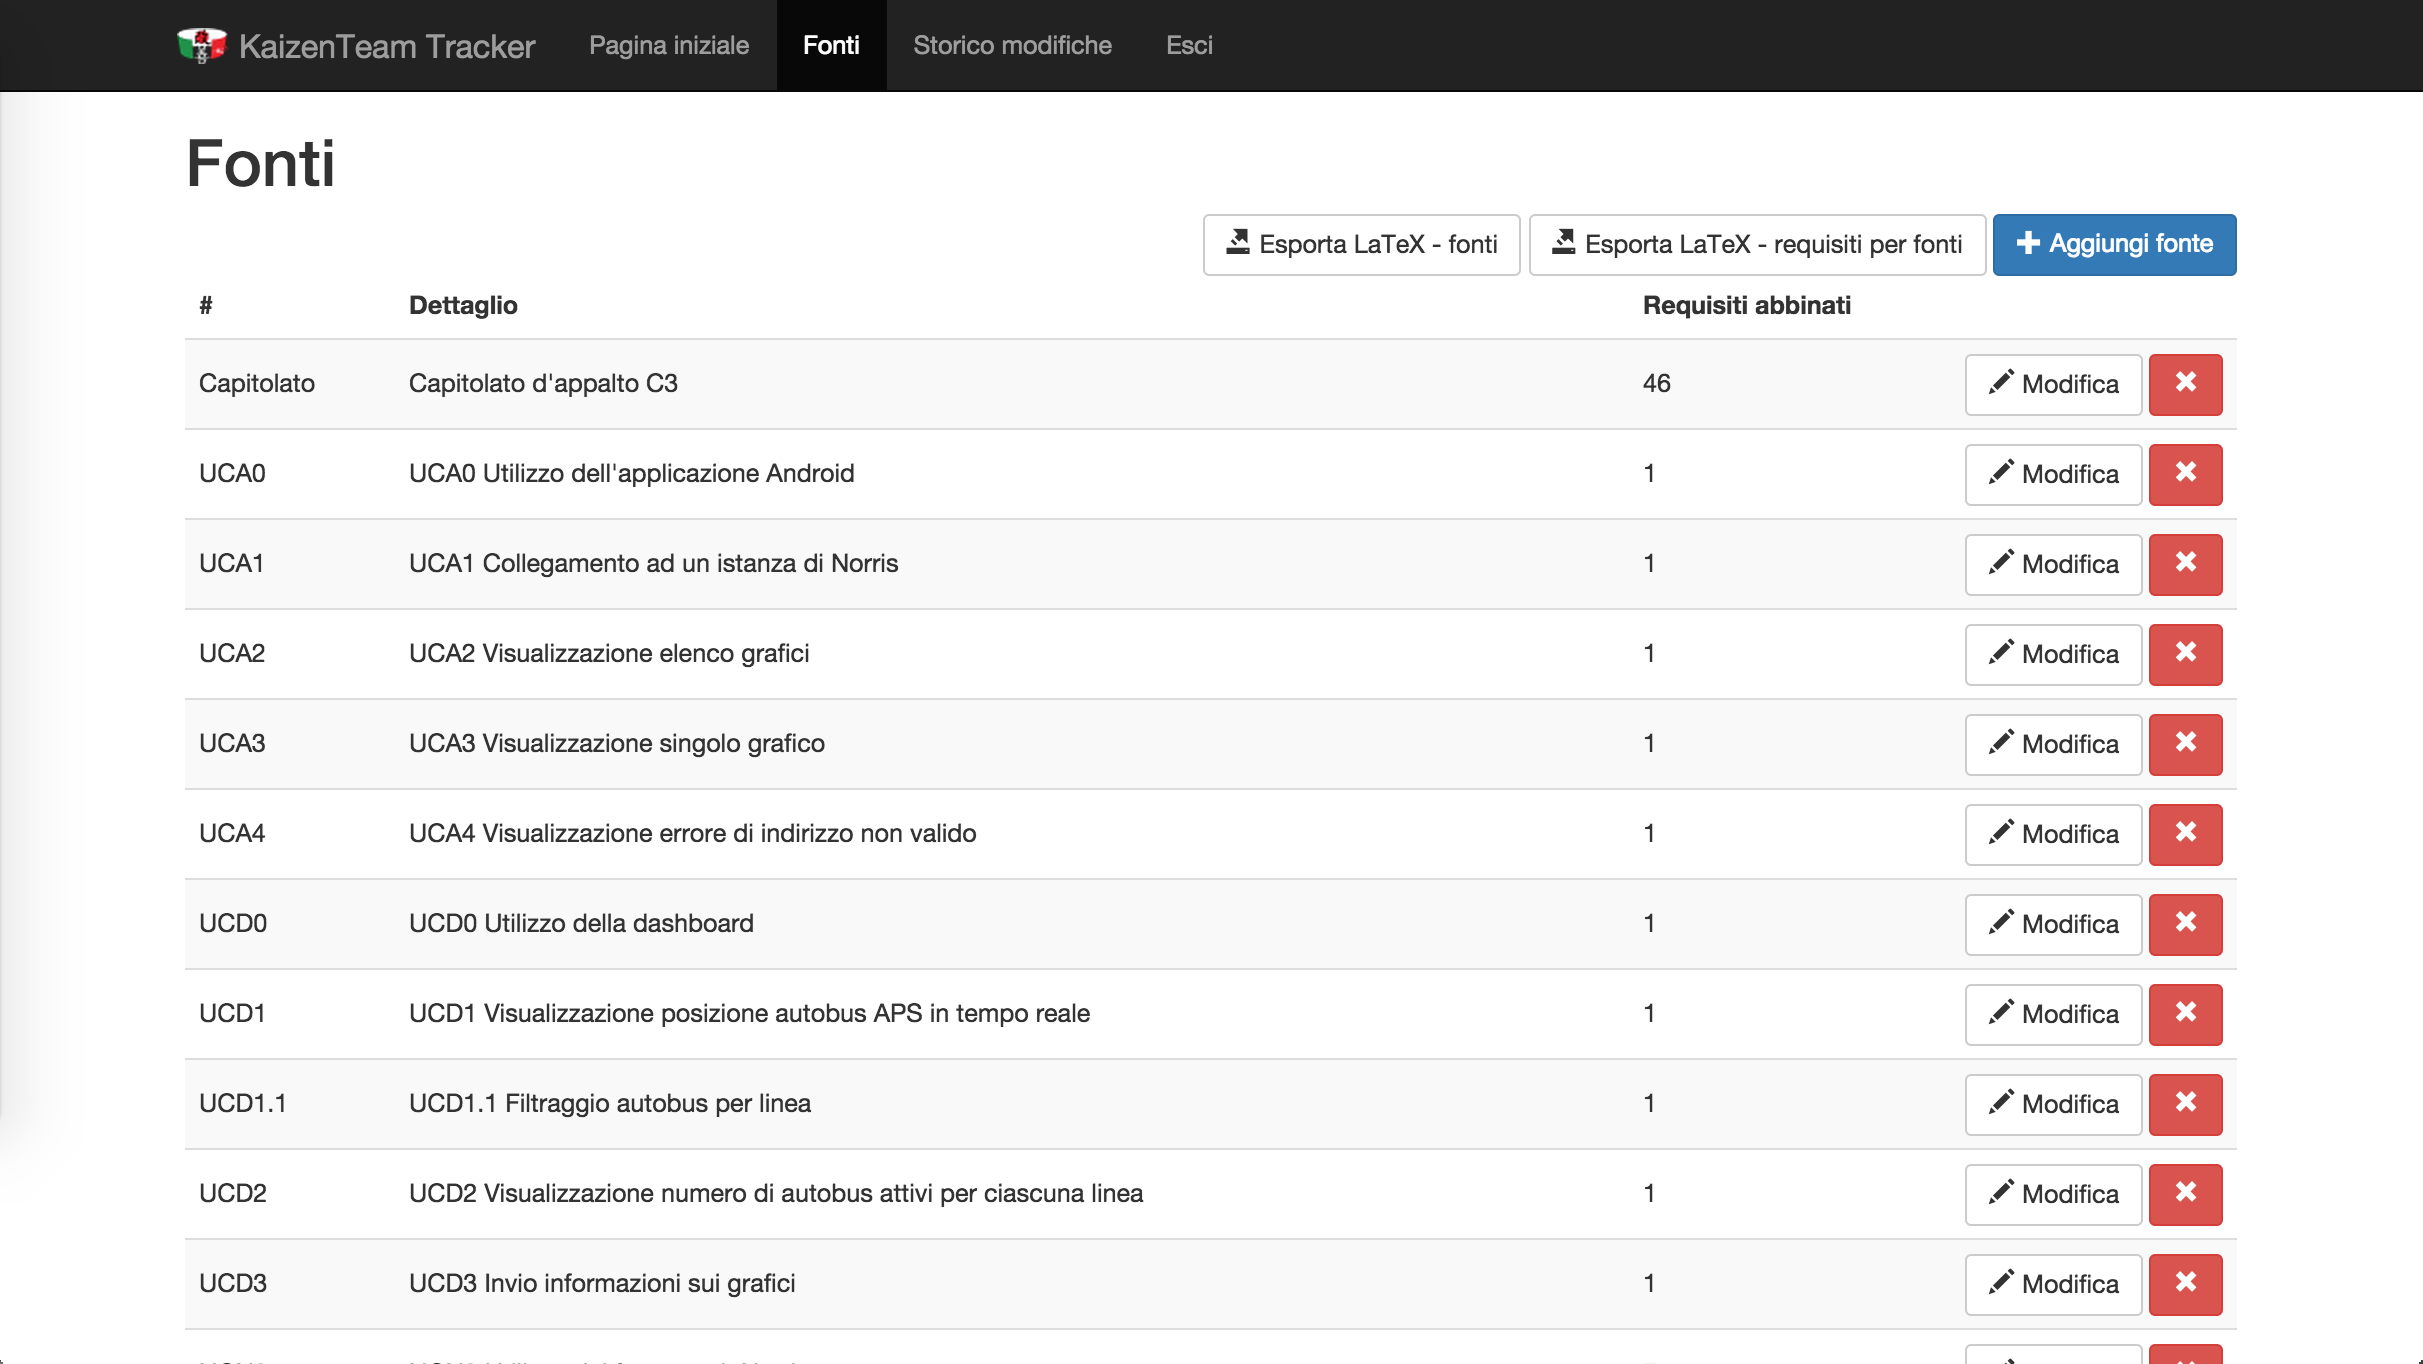
\includegraphics[width=\textwidth]{Pics/TrackerFonti}
	\caption{Tracker - Aggiunta delle fonti}
\end{figure}


\begin{figure}[H]
	\centering
	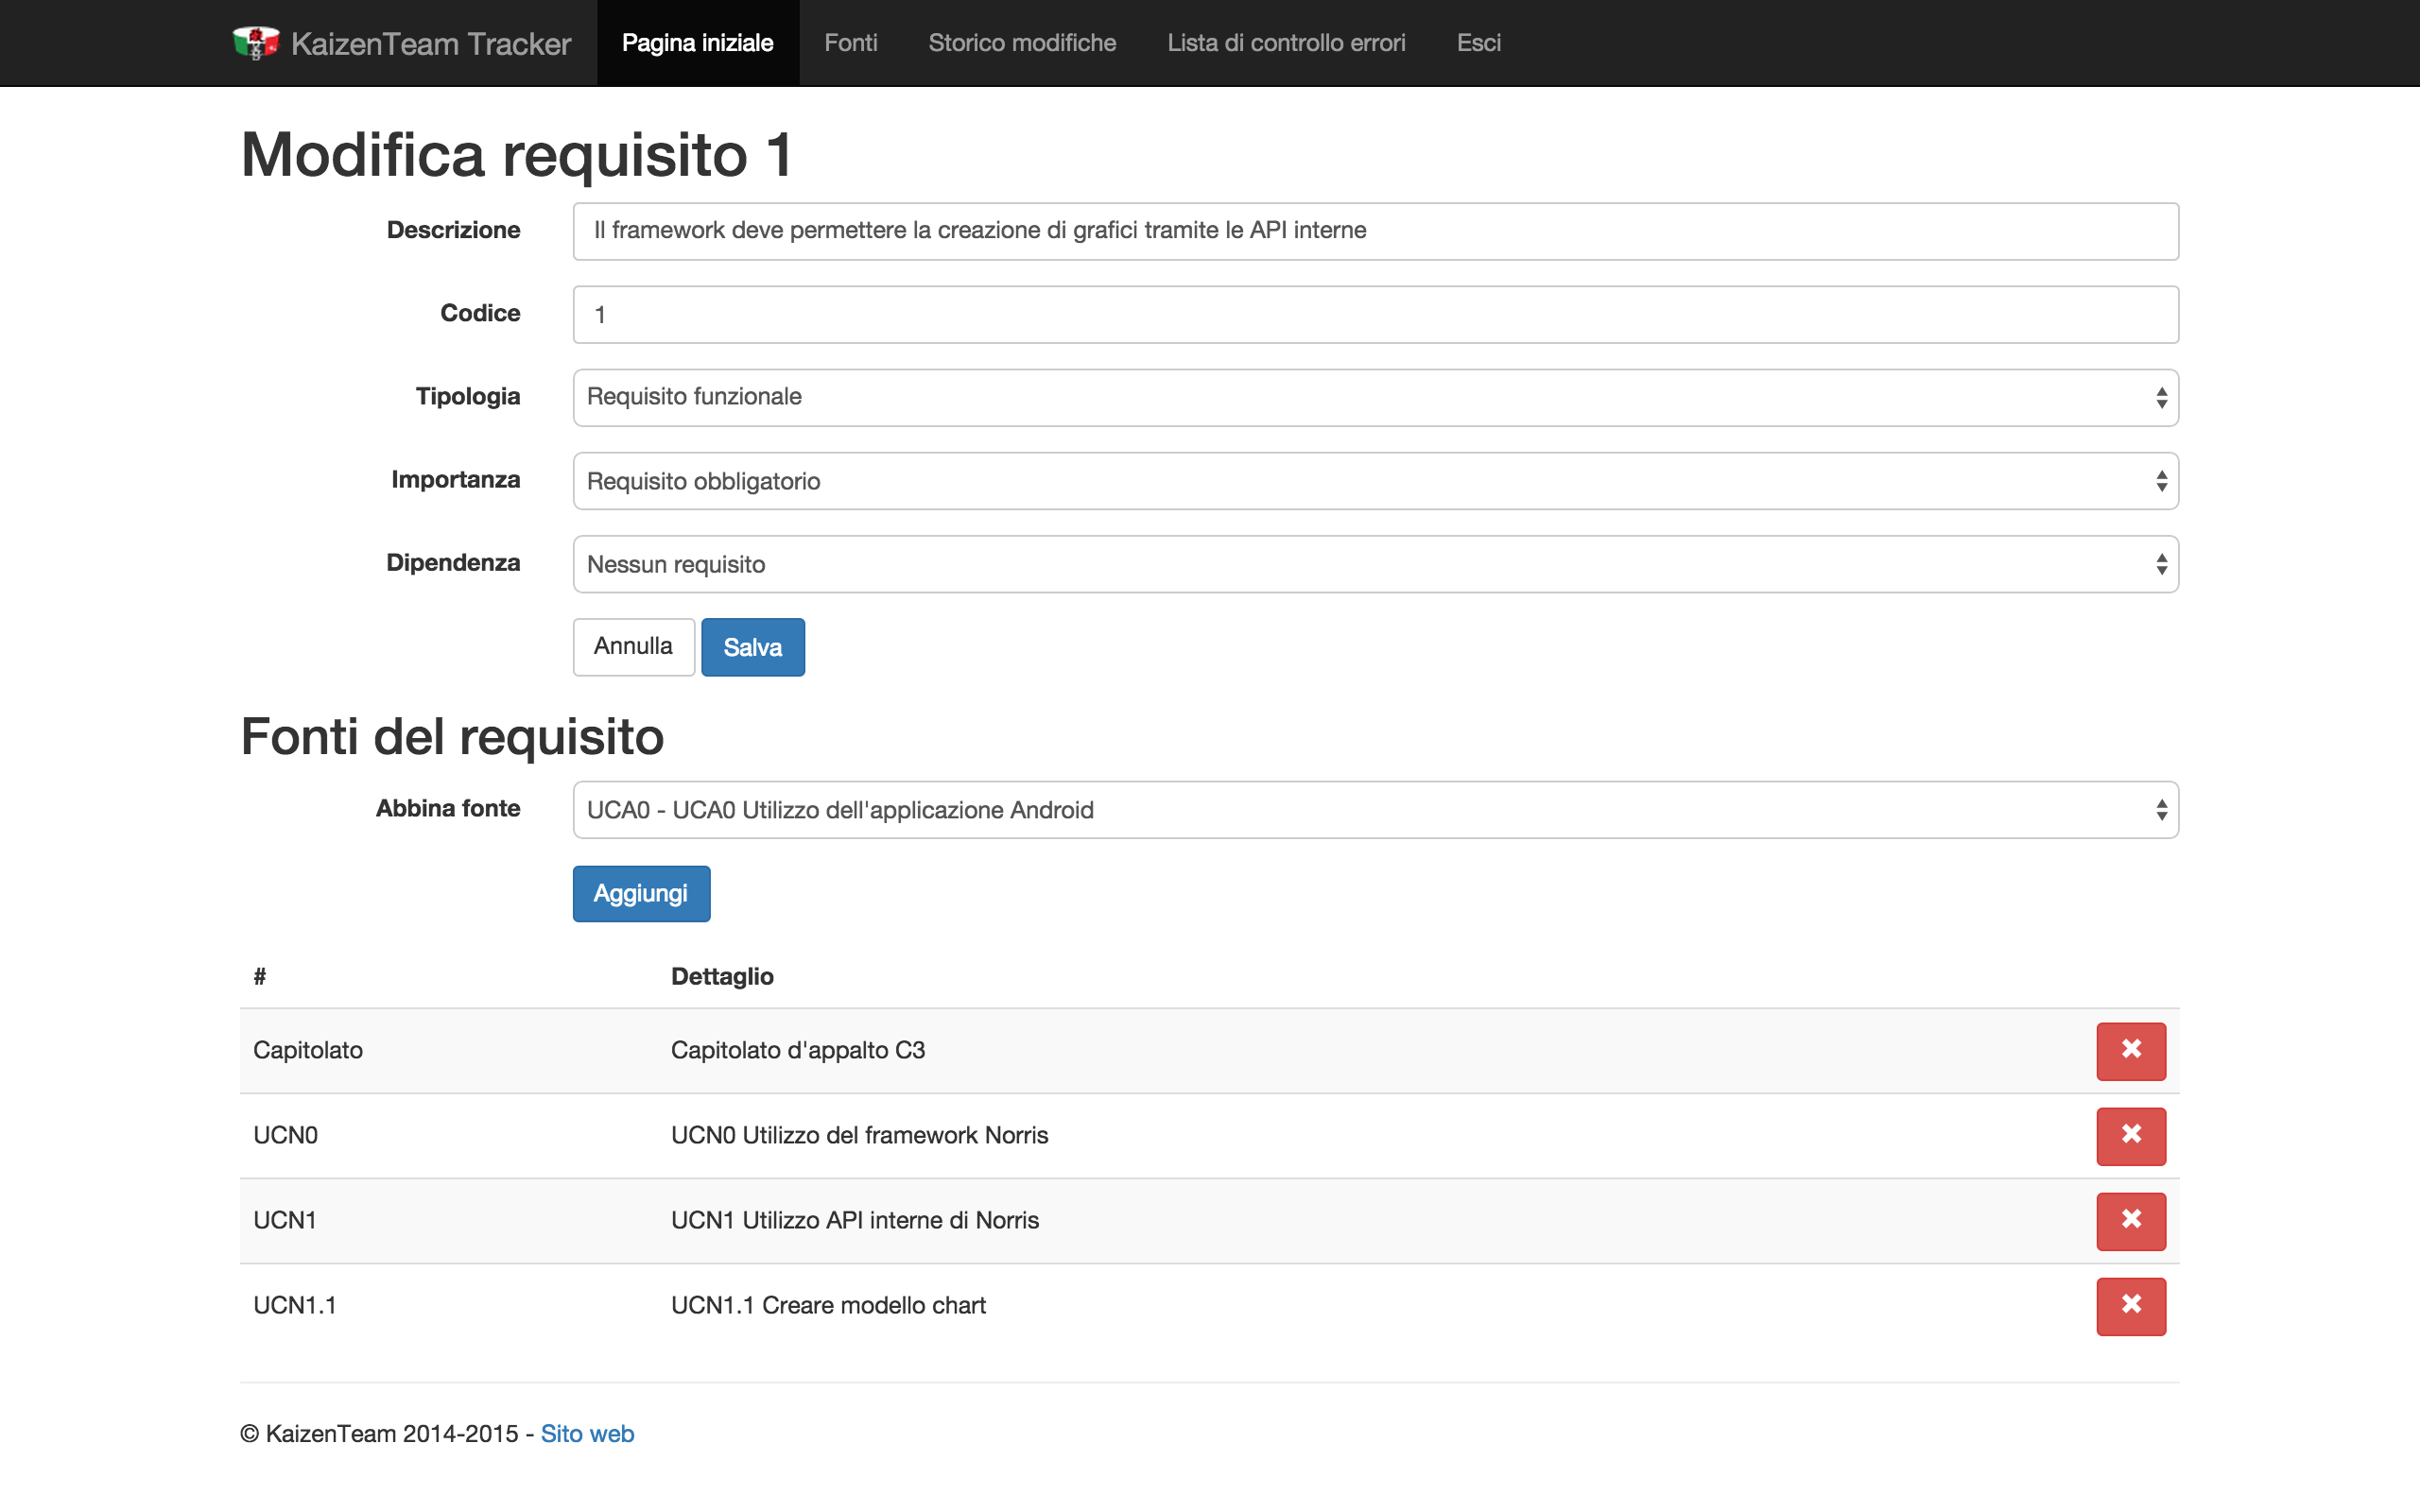
\includegraphics[width=\textwidth]{Pics/TrackerModificaRequisito}
	\caption{Tracker - Modifica di un requisito}
\end{figure}